% ------------------------------------------------------------------------------
% TYPO3 CMS 6.2 LTS - What's New - Chapter "In-Depth Changes" (Italian Version)
%
% @author Roberto Torresani <roberto.torresani@typo3.org>
% @license	Creative Commons BY-NC-SA 3.0
% @link		http://typo3.org/download/release-notes/whats-new/
% @language	Italian
% ------------------------------------------------------------------------------
% Chapter: In-Depth Changes
% ------------------------------------------------------------------------------

\section{Modifiche rilevanti}
\begin{frame}[fragile]
	\frametitle{Modifiche rilevanti}

	\begin{center}\huge{Capitolo 6:}\end{center}
	\begin{center}\huge{\color{typo3darkgrey}\textbf{Modifiche rilevanti}}\end{center}

\end{frame}

% ------------------------------------------------------------------------------
% normalize.css
% ------------------------------------------------------------------------------
% http://forge.typo3.org/issues/47920

\begin{frame}[fragile]
	\frametitle{Modifiche rilevanti}
	\framesubtitle{Normalize.css}

	\begin{itemize}
		\item L'interfaccia utente di backend fa uso di \texttt{normalize.css},\newline
			che permette ai browser di avere tutti gli elementi più coerenti e in linea con gli standard moderni
		\item Moderno, pronto per HTML5, alternativo al CSS tradizionale
		\item Obiettivi di \texttt{normalize.css} sono:

			\begin{itemize}
				\item Mantenere i valori utili del browser invece di cancellarli
				\item Normalizzare gli stili per una vasta gamma di elementi HTML
				\item Correggere i bug e le incoerenze più comuni dei browser
				\item Migliorare l'usabilità con piccoli miglioramenti
				\item Spiegare il codice usando osservazioni e documentazione dettagliata
			\end{itemize}

	\end{itemize}

\end{frame}

% ------------------------------------------------------------------------------
% displayCond options BIT and !BIT
% ------------------------------------------------------------------------------
% http://forge.typo3.org/issues/45514

\begin{frame}[fragile]
	\frametitle{Modifiche rilevanti}
	\framesubtitle{TCA: opzione displayCond BIT e !BIT}

	\lstset{
		basicstyle=\tiny\ttfamily
	}

	\begin{itemize}
		\item Verificare con un campo multivalore \texttt{displayCond} (bitwise)\newline
			\texttt{BIT}: bit è impostato, \texttt{!BIT}: bit \underline{non} è impostato
	\end{itemize}

	\begin{columns}[T]

		\begin{column}{.5\textwidth}

			\advance\leftskip+1cm
			Considerando questo TCA:

			\lstset{xleftmargin=1cm}

			\begin{lstlisting}
				'content' => array(
				  'label' => '...',
				  'config' => array(
				    'type' => 'check',
				    'items' => array(
				      array('Content A', ''),
				      array('Content B', ''),
				      array('Content C', ''),
				    ),
				  )
				),
			\end{lstlisting}

		\end{column}
		\begin{column}{.5\textwidth}

			Esempio:

			\begin{lstlisting}
				'content_a' => array(
				  'label' => '...',
				  'displayCond' => 'FIELD:content:BIT:1',
				  'config' => array(
				    'type' => 'text',
				  )
				),

				'content_b' => array(
				  'label' => '...',
				  'displayCond' => 'FIELD:content:!BIT:2',
				  'config' => array(
				    'type' => 'text',
				  )
				),
			\end{lstlisting}
		\end{column}

	\end{columns}

\end{frame}

% ------------------------------------------------------------------------------
% Automatic language updates for extensions
% ------------------------------------------------------------------------------
% http://forge.typo3.org/issues/43703

\begin{frame}[fragile]
	\frametitle{Modifiche rilevanti}
	\framesubtitle{Aggiornamento lingue}

	\begin{itemize}
		% \item Extbase Command Controller allows to update translations of extensions for selected languages
		\item Extbase Command Controller permette gli aggiornamenti di lingua per le estensioni:

			\begin{lstlisting}
				$GLOBALS['TYPO3_CONF_VARS']['SC_OPTIONS']['extbase']
				  ['commandControllers'][] =
				  'TYPO3\\CMS\\Lang\\Command\\LanguageCommandController';
			\end{lstlisting}

		\item Chiamata di esempio:

			\lstinline!typo3/cli_dispatch.phpsh extbase language:update de,en,fr!

		\item Elenco separato da virgole delle locale (es. \texttt{de,en,fr}) limita l'aggiornamento a queste lingue
		\item Senza questo parametro, tutte le lingue impostate nel modulo "Lingue" sono aggiornate

	\end{itemize}

\end{frame}

% ------------------------------------------------------------------------------
% Migrate system extension manuals to reStructuredText
% ------------------------------------------------------------------------------
% http://forge.typo3.org/issues/50052

\begin{frame}[fragile]
	\frametitle{Modifiche rilevanti}
	\framesubtitle{System Extensions: ReST Manuals}

	\begin{itemize}
		\item Tutti i manuali di sistema sono stati migrati a reStructuredText
		\item I manuali in OpenOffice non sono più usati e sono stati rimossi
		\item ReST è semplice da leggere, what-you-see-is-what-you-get plaintext markup syntax and parser system
		\item I file ReST delle estensioni di sistema si trovano in:\newline
			\texttt{typo3/sysext/<extensionkey>/Documentation/*}

		\item Ulteriori informazioni:

			\begin{itemize}
				\item \url{http://de.wikipedia.org/wiki/ReStructuredText}
				\item \url{http://wiki.typo3.org/ReST}
			\end{itemize}

	\end{itemize}

\end{frame}

% ------------------------------------------------------------------------------
% Support custom translation servers for extensions
% ------------------------------------------------------------------------------
% http://forge.typo3.org/issues/50052

\begin{frame}[fragile]
	\frametitle{Modifiche rilevanti}
	\framesubtitle{Server delle traduzioni personalizzato}

	\begin{itemize}
		\item E' implementato un supporto alla personalizzazione delle traduzioni delle estensione
		\item Con l'uso di XLIFF e un nuovo Segnale/Slot,\newline
			questo diventa molto semplice (vedi la prossima slide per un esempio)
		\item Un possibile server di traduzione: \textbf{Pootle}

			\begin{itemize}
				\item gestione traduzioni online con interfaccia per le traduzioni
				\item scritto in Python/Django
				\item originariamente sviluppato e rilasciato da \url{translate.org.za}
				\item licenza GNU GPL
			\end{itemize}

	\end{itemize}

\end{frame}

% ------------------------------------------------------------------------------
% Support custom translation servers for extensions
% ------------------------------------------------------------------------------
% http://forge.typo3.org/issues/50052

\begin{frame}[fragile]
	\frametitle{Modifiche rilevanti}
	\framesubtitle{Server delle traduzioni personalizzato}

	Esempio: \texttt{EXT:myextension/localconf.php}

	\lstset{
		basicstyle=\tiny\ttfamily
	}

	\begin{lstlisting}
		/**
		 * @var \TYPO3\CMS\Extbase\SignalSlot\Dispatcher $signalSlotDispatcher
		 */
		$signalSlotDispatcher =
		  \TYPO3\CMS\Core\Utility\GeneralUtility::makeInstance(
		    'TYPO3\\CMS\\Extbase\\SignalSlot\\Dispatcher');

		$signalSlotDispatcher->connect(
		  'TYPO3\\CMS\\Lang\\Service\\UpdateTranslationService',
		  'postProcessMirrorUrl',
		  'Company\\Extension\Slots\\CustomMirror',
		  'postProcessMirrorUrl'
		);
	\end{lstlisting}

\end{frame}

% ------------------------------------------------------------------------------
% Support custom translation servers for extensions
% ------------------------------------------------------------------------------
% http://forge.typo3.org/issues/50052

\begin{frame}[fragile]
	\frametitle{Modifiche rilevanti}
	\framesubtitle{Server delle traduzioni personalizzato}

	Esempio: \texttt{EXT:myextension/Classes/Slots/CustomMirror.php}

	\lstset{
		basicstyle=\tiny\ttfamily
	}

	\begin{lstlisting}
		<?php
		namespace Company\Extensions\Slots;
		class CustomMirror {

		  /**
		   * @var string
		   */
		  protected static $extKey = 'myextension';

		  public function postProcessMirrorUrl($extensionKey, &$mirrorUrl) {
		    if ($extensionKey === self::$extKey) {
		      $mirrorUrl = 'http://example.com/typo3-packages/';
		    }
		  }

		}
	\end{lstlisting}

\end{frame}

% ------------------------------------------------------------------------------
% Support custom translation servers for extensions
% ------------------------------------------------------------------------------
% http://forge.typo3.org/issues/50052

\begin{frame}[fragile]
	\frametitle{Modifiche rilevanti}
	\framesubtitle{Server delle traduzioni personalizzato}

	Struttura dei file e directory sul server:

	\begin{lstlisting}
		http://example.com/typo3-packages/
		 `-- <first-letter-of-extension-key>
		     `-- <second-letter-of-extension-key>
		         `-- <extension-key>-l10n
		             |-- <extension-key>-l10n-de.zip
		             |-- <extension-key>-l10n-fr.zip
		             |-- <extension-key>-l10n-it.zip
		             `-- <extension-key>-l10n.xml
	\end{lstlisting}

	Un esempio:

	\begin{lstlisting}
		http://example.com/typo3-packages/m/y/myextension-l10n/myextension-l10n.xml
	\end{lstlisting}

\end{frame}

% ------------------------------------------------------------------------------
% Support custom translation servers for extensions
% ------------------------------------------------------------------------------
% http://forge.typo3.org/issues/50052

\begin{frame}[fragile]
	\frametitle{Modifiche rilevanti}
	\framesubtitle{Server delle traduzioni personalizzato}

	Esempio: \texttt{<extension-key>-l10n.xml}

	\lstset{
		basicstyle=\tiny\ttfamily
	}

	\begin{lstlisting}
		<?xml version="1.0" standalone="yes" ?>
		  <TERlanguagePackIndex>
		    <meta>
		      <timestamp>1374841386</timestamp>
		      <date>2013-07-26 14:23:06</date>
		    </meta>
		    <languagePackIndex>
		    <languagepack language="de">
		      <md5>1cc7046c3b624ba1fb1ef565343b84a1</md5>
		    </languagepack>
		    <languagepack language="fr">
		     <md5>f00f73ae5c43cb68392e6c508b65de7a</md5>
		    </languagepack>
		    <languagepack language="it">
		     <md5>cd59530ce1ee0a38e6309544be6bcb3d</md5>
		    </languagepack>
		  </languagePackIndex>
		</TERlanguagePackIndex>
	\end{lstlisting}

\end{frame}

% ------------------------------------------------------------------------------
% Automatic import of t3d files for extensions
% ------------------------------------------------------------------------------
% http://forge.typo3.org/issues/51437

\begin{frame}[fragile]
	\frametitle{Modifiche rilevanti}
	\framesubtitle{Importazione automatica file t3d}

	\begin{itemize}
		\item Le estensioni possono importare automaticamente i \textbf{pacchetti t3d} \newline
			durante l'installazione della stessa.
		\item I file t3d contengono informazioni come dati, relazioni, file, ecc.
		\item I file t3d devono essere nominati \texttt{data.t3d} e posizionati in:\newline
			\texttt{EXT:myextension/Initialisation/}

		\item L'importazione avviene \underline{una sola} volta\newline
			(anche se l'estensione viene reinstallata in seguito)

	\end{itemize}

\end{frame}

% ------------------------------------------------------------------------------
% Automatic import of files for extensions
% ------------------------------------------------------------------------------
% http://forge.typo3.org/issues/51446

\begin{frame}[fragile]
	\frametitle{Modifiche rilevanti}
	\framesubtitle{Importazione automatica dei file}

	\begin{itemize}
		\item Le estensioni possono importare automaticamente dei \textbf{file}\newline
			durante l'installazione della stessa.
		\item I file sono copiati in:\newline
			\texttt{fileadmin/<extensionkey>/}
		\item I file devono essere posizionati in:\newline
			\texttt{EXT:myextension/Initialisation/Files/...}

		\item L'importazione avviene \underline{una sola} volta\newline
			(anche se l'estensione viene reinstallata in seguito)

	\end{itemize}

\end{frame}

% ------------------------------------------------------------------------------
% Use an extension as repository
% ------------------------------------------------------------------------------
% http://forge.typo3.org/issues/51835

\begin{frame}[fragile]
	\frametitle{Modifiche rilevanti}
	\framesubtitle{Utilizzare un estensione come archivio}

	\begin{itemize}
		\item A volte le estensioni dipendono da versioni personalizzate di altre estensioni o da estensioni che non sono state rilasciate nell'archivio ufficiale delle estensioni di TYPO3 (TER)
		\item Per risolvere questo problema, le estensioni possono essere rilasciate con "altre" estensioni.
		\item Queste devono essere posizionati in (scompattate):\newline
			\texttt{EXT:myextension/Initialisation/Extensions/...}

		\item Al momento dell'installazione le estensioni sono copiate in:\newline
			\texttt{typo3conf/ext/}

		\item A questo punto, le dipendenze sono risolte

	\end{itemize}

\end{frame}

% ------------------------------------------------------------------------------
% CLI command to install/uninstall extensions
% ------------------------------------------------------------------------------
% http://forge.typo3.org/issues/51629

\begin{frame}[fragile]
	\frametitle{Modifiche rilevanti}
	\framesubtitle{Installare/disinstallare estensioni via CLI}

	\begin{itemize}
		\item Installare e disinstallare le estensioni da linea di comando (CLI)
		\item Esempi:
			\lstinline!typo3/cli_dispatch.phpsh extbase extension:install <extensionkey>!
			\lstinline!typo3/cli_dispatch.phpsh extbase extension:uninstall <extensionkey>!

		\item Nota: è necessario l'utente di backend \textbf{\_cli\_lowlevel}
	\end{itemize}

\end{frame}

% ------------------------------------------------------------------------------
% Enable/disable cascading deletion of child elements
% ------------------------------------------------------------------------------
% http://forge.typo3.org/issues/50391

\begin{frame}[fragile]
	\frametitle{Modifiche rilevanti}
	\framesubtitle{Cancellazione di elementi figli a cascata}

	\begin{itemize}
		\item Il TCA ora dispone di una funzionalità per abilitare/disabilitare la cancellazione degli elementi figli a cascata
		\item La relazione deve essere di tipo "inline"
		\item Il valore predefinito è \texttt{TRUE} (la cancellazione degli elementi figli è attiva)
		\item Esempio (disabilitare la cancellazione degli elementi figli):

			\begin{lstlisting}
				...
				'type' => 'inline',
				'foreign_table' => ...,
				  'behaviour' => array(
				    'enableCascadingDelete' => 0
				  )
				  ...
				)
				...
			\end{lstlisting}

	\end{itemize}

\end{frame}

% ------------------------------------------------------------------------------
% Multiple category fields per table
% ------------------------------------------------------------------------------
% http://forge.typo3.org/issues/51921

\begin{frame}[fragile]
	\frametitle{Modifiche rilevanti}
	\framesubtitle{Campi "category" multipli per tabella}

	\begin{itemize}
		\item In TYPO3 < 6.2, è possibile fare solo \underline{una} chiamata \texttt{makeCategorizable()} per tabella
			(chiamate multiple sovrascrivono la dichiarazione precedente del campo "category")
		\item Da TYPO3 >= 6.2, sono possibili campi "category" multipli per tabella
		\item Esempio:

			\begin{lstlisting}
				\TYPO3\CMS\Core\Utility\ExtensionManagementUtility::makeCategorizable(
				  $extensionKey,
				  $tableName,
				  $fieldName = 'categories',
				  $options = array(
				  	'label' => 'my category'
				) );
			\end{lstlisting}

		\item Per "category" si possono impostare etichette personalizzate nella matrice array \texttt{\$options}

	\end{itemize}

\end{frame}

% ------------------------------------------------------------------------------
% Backend layout data providers
% ------------------------------------------------------------------------------
% http://forge.typo3.org/issues/37208

\begin{frame}[fragile]
	\frametitle{Modifiche rilevanti}
	\framesubtitle{Fornitore di dati per Backend Layout}

	\begin{itemize}
		\item In TYPO3 < 6.2, i "backend layouts" sono registrati nel DB come record normali
		\item Da TYPO3 >= 6.2, i cosidetti \emph{data providers} possono essere definiti\newline
			\small(per esempio abilitare le estensioni ad inviare le proprie definizioni di "backend layout" da file statici)\normalsize

		\item I fornitori di dati devono implementare le interfacce:\newline
			\smaller\texttt{
				TYPO3\textbackslash\textbackslash
				CMS\textbackslash\textbackslash
				Backend\textbackslash\textbackslash
				View\textbackslash\textbackslash
				BackendLayout\textbackslash\textbackslash
				DataProviderInterface}\normalsize

		\item e possono essere registrate da:

			\begin{lstlisting}
				$GLOBALS['TYPO3_CONF_VARS']['SC_OPTIONS']
				  ['BackendLayoutDataProvider'][$_EXTKEY] = 'Classname';
			\end{lstlisting}


	\end{itemize}

\end{frame}

% ------------------------------------------------------------------------------
% Backend layout data providers
% ------------------------------------------------------------------------------
% http://forge.typo3.org/issues/37208

\begin{frame}[fragile]
	\frametitle{Modifiche rilevanti}
	\framesubtitle{Fornitore di dati per Backend Layout}

	\begin{itemize}
		\item Nuove API per manipolare i fornitori di dati per "backend layout":

			\begin{lstlisting}
				'itemsProcFunc' => 'TYPO3\\CMS\\Backend\\View\\
				  BackendLayoutView->addBackendLayoutItems'
			\end{lstlisting}

			\begin{lstlisting}
				getBackendLayoutView()->getSelectedCombinedIdentifier($id);
				getBackendLayoutView()->getSelectedBackendLayout();
			\end{lstlisting}

		\item Nuove opzioni PageTSconfig per escludere "backend layouts":

			\begin{lstlisting}
				options.backendLayout.exclude = default_1, my_extension__headerLayout
			\end{lstlisting}

	\end{itemize}

\end{frame}

% ------------------------------------------------------------------------------
% Filter for multiple value selector
% ------------------------------------------------------------------------------
% http://forge.typo3.org/issues/49739

\begin{frame}[fragile]
	\frametitle{Modifiche rilevanti}
	\framesubtitle{Selezione di valori multipli (1)}

	\lstset{
		basicstyle=\tiny\ttfamily
	}

	\begin{itemize}
		\item Filtra gli elementi disponibili in un elemento multi-select (TCA)
		\item Esempio: abilitare un campo testo ad usare delle ricerche di parole predefinite e filtrate che l'utente può scegliere da un elemento a tendina

		\item Per utilizzare questa nuova funziona, impostare TCA adeguatamente\newline
			(es. nel file \texttt{typo3conf/extTables.php}):


			\begin{lstlisting}
				$GLOBALS['TCA']['fe_users']['columns']['usergroup']['config']
				  ['enableMultiSelectFilterTextfield'] = TRUE;

				$GLOBALS['TCA']['fe_users']['columns']['usergroup']['config']
				  ['multiSelectFilterItems'] = array(

				  array('',     'show all'),  // no filter
				  array('test', 'test'),      // first value: filter, second value: label

				  array(
				    'TYPO3',
				    'LLL:EXT:myext/Resources/Private/Language/locallang_db.xlf:tx_myext.label.typo3'
				  ),
				);
			\end{lstlisting}

	\end{itemize}

\end{frame}

% ------------------------------------------------------------------------------
% Filter for multiple value selector
% ------------------------------------------------------------------------------
% http://forge.typo3.org/issues/49739

\begin{frame}[fragile]
	\frametitle{Modifiche rilevanti}
	\framesubtitle{Selezione di valori multipli (2)}

	Il risultato sarà simile al seguente:

	\begin{figure}
		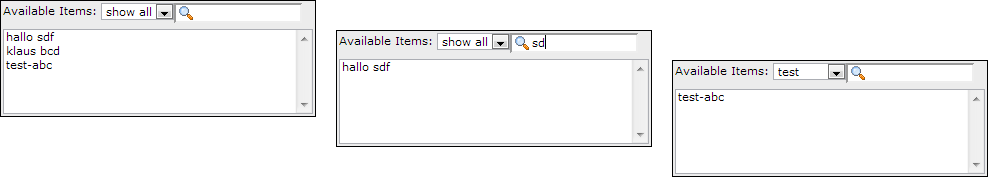
\includegraphics[width=1\linewidth]{Images/InDepthChanges/MultipleValueSelector.png}
	\end{figure}

\end{frame}

% ------------------------------------------------------------------------------
% Improved caching framework by introducing cache groups
% (slide added in March 2014)
% ------------------------------------------------------------------------------
% http://forge.typo3.org/issues/54991

\begin{frame}[fragile]
	\frametitle{Modifiche rilevanti}
	\framesubtitle{Gruppi di cache (1)}

	\begin{itemize}
		\item Il core di TYPO3 usa due tipi di cache:

			\begin{itemize}
				\item \textbf{cache relativa al sistema}:
				cache di caricamento classi, cache delle configurazioni, l10n\_cache, extbase\_object, extbase\_reflection, ecc.
				\item \textbf{cache relativa al frontend}:
				cHash cache, cache delle pagine, cache delle sezioni di pagina
			\end{itemize}

		\item In TYPO3 < 6.2, \textit{cancella tutte le caches} svuota \underline{tutte} le cache, ma non è l'ideale

		\item In TYPO3 >= 6.2, il core utilizza due gruppi di cache:\newline
			"\textbf{pagine}", con tutte le cache relative alle pagine, e "\textbf{sistema}", cache che viene utilizzato nella fase di compilazione e configurazione

	\end{itemize}

	\begin{figure}
		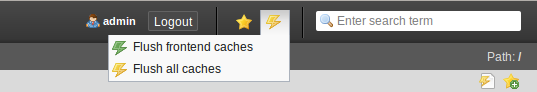
\includegraphics[width=0.5\linewidth]{Images/InDepthChanges/CacheGroups.png}
	\end{figure}

\end{frame}

% ------------------------------------------------------------------------------
% Improved caching framework by introducing cache groups
% (slide added in March 2014)
% ------------------------------------------------------------------------------
% http://forge.typo3.org/issues/54991

\begin{frame}[fragile]
	\frametitle{Modifiche rilevanti}
	\framesubtitle{Gruppi di cache (2)}

	\lstset{
		basicstyle=\tiny\ttfamily
	}

	\begin{itemize}

		\item Opzioni rilevanti di configurazione:\newline
			\smaller(nei file: \texttt{LocalConfiguration.php}/\texttt{DefaultConfiguration.php})\normalsize

			\begin{lstlisting}
			'cache_hash' => array(
			  'frontend' => 'TYPO3\CMS\Core\Cache\Frontend\VariableFrontend',
			  'backend' => 'TYPO3\CMS\Core\Cache\Backend\Typo3DatabaseBackend',
			  'options' => array(),
			  'groups' => array('pages', 'all')
			),
			\end{lstlisting}

		\item Il comando "\textit{Flush all caches}" non cancella più la cache relativa al sistema
			(solo "Cancella la cache delle configurazioni" o lo Strumento di installazione svuota questa cache)
		\item Una nuova opzione userTSconfig abilita gli utenti non amministratori a cancellare la cache di sistema:\newline
			\smaller\texttt{options.clearCache.system = 1}\normalsize

		\breakingchange

	\end{itemize}

\end{frame}

% ------------------------------------------------------------------------------
% TCA: limit number of ticked checkboxes
% (slide added in March 2014)
% ------------------------------------------------------------------------------
% http://forge.typo3.org/issues/55187
% http://forge.typo3.org/issues/55188 (documentation: TCA reference)

\begin{frame}[fragile]
	\frametitle{Modifiche rilevanti}
	\framesubtitle{TCA: Numero di checkbox selezionabili}

	\lstset{
		basicstyle=\tiny\ttfamily
	}

	\begin{itemize}
		\item TCA permette di impostare il numero di checkbox selezionabili

			\begin{itemize}
				\item \texttt{maximumRecordsChecked}:\newline
					numero massimo di record a livello di sistema
				\item \texttt{maximumRecordsCheckedInPid}:\newline
					numero massimo di record a livello di PID (ID genitore)
			\end{itemize}

		\item Se un utente di BE eccede il numero massimo, la seleziona aggiuntiva viene azzerata fino a quando un altro record è deselezionato

		\item Esempio:

			\begin{lstlisting}
				$tcaConfiguration = array(
				  'type' => 'check',
				  'eval' => 'maximumRecordsChecked',
				  'validation' => array(
				    'maximumRecordsChecked' => 5
				  )
				);
			\end{lstlisting}

	\end{itemize}

\end{frame}

% ------------------------------------------------------------------------------
% TCA: Introduce MM_oppositeUsage property
% (slide added in March 2014)
% ------------------------------------------------------------------------------
% http://forge.typo3.org/issues/56061
% http://forge.typo3.org/issues/56123 (documentation: TCA reference)

\begin{frame}[fragile]
	\frametitle{Modifiche rilevanti}
	\framesubtitle{TCA: proprietà \texttt{MM\_oppositeUsage}}

	\lstset{
		basicstyle=\tiny\ttfamily
	}

	\begin{itemize}
		\item Nella copia di un record \texttt{sys\_category}, un nuovo riferimento MM è creato, ma senza impostare il "fieldname"
		\item Questo valore è sostanzialmente definito dall'altra entità con \texttt{MM\_match\_fields}, ma non è possibile accedervi
		\item Per risolvere questo problema, una nuova proprietà \texttt{MM\_oppositeUsage} è stata introdotta nel TCA:

			\begin{lstlisting}
				'config' => array(
				  'allowed' => '*',
				  'MM' => 'tx_myextension_first_second_mm',
				  'MM_oppositeUsage' => array(
				    'tt_content' => array('somefield'),
				    'tx_myextension_domain_model' => array('some_property'),
				  ),
				),
			\end{lstlisting}

	\end{itemize}

\end{frame}

% ------------------------------------------------------------------------------
% Miscellaneous
% ------------------------------------------------------------------------------
% http://forge.typo3.org/issues/49037 (Custom record list in element browser)
% http://forge.typo3.org/issues/36505 (Increase size of be_groups.subgroup field)
% http://forge.typo3.org/issues/49270 (Merge extensions TS/Template)

\begin{frame}[fragile]
	\frametitle{Modifiche rilevanti}
	\framesubtitle{Varie}

	\begin{itemize}

		\item \textbf{Lista dei record personalizzato:}\newline
			\small
				Un istanza personalizzata delle liste di record può essere utilizzata nella navigazione degli elementi
			\normalsize

		\item \textbf{Più sottogruppi:}\newline
			\small
				l'attributo \texttt{subgroup} nella tabella del DB \texttt{be\_groups} cambia da \texttt{varchar(250)} a \texttt{text}, il che permette un numero maggiore di sottogruppi (utenti/gruppi di backend)
			\normalsize

		\item \textbf{Estensioni TS/Template unite:}\newline
			\small
				Tecnicamente, "WEB > Template" è stata suddivisa in varie estensioni (tstemplate\_ceditor, tstemplate\_info, tstemplate\_objbrowser and tstemplate\_analyzer). Tutte queste estensioni sono state unite in un unica estensione: "tstemplate"
			\normalsize

	\end{itemize}
	
\end{frame}

% ------------------------------------------------------------------------------
% Miscellaneous
% ------------------------------------------------------------------------------
% http://forge.typo3.org/issues/49721 (Add label_userFunc_options support to BackendUtility)
% http://forge.typo3.org/issues/50441 (Add a timestamp when downloading an extension)
% http://forge.typo3.org/issues/51352 (Force saltedpasswords for Backend)

\begin{frame}[fragile]
	\frametitle{Modifiche rilevanti}
	\framesubtitle{Varie}

	\begin{itemize}

		\item \textbf{label\_userFunc\_options:}\newline
			\small
				\texttt{label\_userFunc\_options} è stata aggiunta a \texttt{BackendUtility}
			\normalsize

		\item \textbf{Nomi dei file delle estenzioni:}\newline
			\small
				Quando si scarica un estensione nel "Gestore delle estensioni", il nome del file contiene timestamp (anno, mese, giorno e ora):\newline
				\texttt{<extensionKey>\_<version>\_<timestamp>.zip}\newline
				\texttt{myextension\_1.0.0\_201312102359.zip}
			\normalsize

		\item \textbf{EXT:saltedpasswords:}\newline
			\small
				L'estensione EXT:saltedpasswords è un estensione di sistema e abilitata di default.
				Questo forza la "salted hashes" per l'autenticazione di backend. Lo "Strumento di installazione" verifica le impostazioni e le adatta se necessario.
			\normalsize

	\end{itemize}
	
\end{frame}

% ------------------------------------------------------------------------------
% Miscellaneous
% ------------------------------------------------------------------------------
% http://forge.typo3.org/issues/51138 (Allow SignalSlots to modify arguments)
% http://forge.typo3.org/issues/31996 (Transfer query parameters in preview)
% http://forge.typo3.org/issues/52630 (TCEforms PlaceHolder works recursively now)

\begin{frame}[fragile]
	\frametitle{Modifiche rilevanti}
	\framesubtitle{Varie}

	\begin{itemize}

		\item \textbf{SignalSlots per modificare i parametri:}\newline
			\small
				I parametri passati a SignalSlots dispatcher possono essere modificati e il dispatcher ritorna i parametri (modificati) come li ha ricevuti al fine di mantenere intatto il concatenamento.
			\normalsize

		\item \textbf{Anteprima dei workspace:}\newline
			\small
				I parametri delle query sono passati al workspace in anteprima ora. Questo era un problema in TYPO3 < 6.2, dove non funzionava correttamente il passaggio di parametri personalizzati alle estensioni.
			\normalsize

		\item \textbf{Caratteristica PlaceHolder di TCEforms:}\newline
			\small
				Introdotto in TYPO3 CMS 4.7, le funzionalità PlaceHolder di TCEforms possono funzionare ricorsivamente ora (es. z.B. \texttt{\_\_row|uid\_foreign|field}).
			\normalsize

	\end{itemize}
	
\end{frame}

% ------------------------------------------------------------------------------
% Miscellaneous
% ------------------------------------------------------------------------------
% http://forge.typo3.org/issues/14730 (Support for proxy NTLM authentication)
% http://forge.typo3.org/issues/49667 (Enable double-resolution icons in SpriteGenerator)

\begin{frame}[fragile]
	\frametitle{Modifiche rilevanti}
	\framesubtitle{Varie}

	\begin{itemize}

		\item \textbf{Doppia risoluzione delle icone:}\newline
			\small
				SpriteManager supporta l'alta risoluzione delle icone ora: è generato un secondo sprite con dimensione doppie delle icone (un secondo file con suffisso "@x2.png"). CSS3 assicura che il file in alta risoluzione è caricato dai dispositivi che lo supportano\newline
				(questo non ha influenza sulle performance degli altri dispositivi).
			\normalsize

		\item \textbf{Autenticazione proxy NTLM:}\newline
			\small
				E' stato aggiunto il supporto per l'autenticazione proxy NTLM (\textbf{NT} \textbf{L}AN \textbf{M}anager: suite di protocolli di sicurezza di Microsoft). Questa funzionalità può essere attivata nello "Strumento di installazione":\newline
			\normalsize
			\smaller
				\texttt{\$GLOBALS['TYPO3\_CONF\_VARS']['SYS']['curlProxyNTLM']}\newline
				\emph{(a proposito: questa funzionalità è stata richiesta più di 8 anni fa :-)}
			\normalsize

	\end{itemize}
	
\end{frame}

% ------------------------------------------------------------------------------
% Miscellaneous
% (slide added in March 2014)
% ------------------------------------------------------------------------------
% http://forge.typo3.org/issues/14730 (Support for proxy NTLM authentication)

\begin{frame}[fragile]
	\frametitle{Modifiche rilevanti}
	\framesubtitle{Varie}

	\begin{itemize}

		\item \textbf{Di default cookieHttpOnly:}\newline
			\small
				Al fine di rendere il cookie di sessione accessibile solo via protocollo HTTP, \texttt{cookieHttpOnly} è ora attivo di default.\newline
				Questo significa che i cookie "fe\_typo\_user" e "be\_typo\_user" non sono accessibili da linguaggi di scripting (es. JavaScript), migliorando la protezione contro attacchi XSS (\textit{cross site scripting}). Alcuni vecchi browser non supportano questa funzionalità.
			\normalsize

                \item \textbf{Pulizia delle tabelle del database:}\newline
                        \small
                                Sono stati rimossi i seguenti campi dalle tabelle del DB \texttt{tt\_content} (non usate da TYPO3 4.0):
                                \texttt{text\_align}, \texttt{text\_face}, \texttt{text\_size}, \texttt{text\_color}, \texttt{text\_properties}.
                        \normalsize

	\end{itemize}
	
\end{frame}

% ------------------------------------------------------------------------------

% ------------------------------------------------------------------------------
% Miscellaneous
% (slide added in March 2014)
% ------------------------------------------------------------------------------
% https://forge.typo3.org/issues/55190 (Move Tidy functionality to a TER extension)

\begin{frame}[fragile]
        \frametitle{Modifiche rilevanti}
        \framesubtitle{Varie}

        \begin{itemize}

                \item \textbf{Rimosso HTML Tidy:}\newline
                        \small
                                La funzionalità \textit{HTML Tidy} è stata rimossa dal core di TYPO3. Può essere riaggiunta installando EXT:tidy dal TER.
                        \normalsize

                \item \textbf{Rimosso dontSetCookie:}\newline
                        \small
				Visto che il cookie "fe\_typo\_user" è usato solo se richiesto (e non sempre), dallo "strumento di installazione" è stata rimossa l'opzione \texttt{dontSetCookie}.
                        \normalsize

                \item \textbf{Rimossi gli script "Wizard":}\newline
                        \small
                                Rimossi i seguenti script "wizard":
                                \texttt{typo3/wizard\_add.php}, \texttt{typo3/wizard\_colorpicker.php}, \texttt{typo3/wizard\_edit.php}, \texttt{typo3/wizard\_forms.php}, \texttt{typo3/wizard\_list.php}, \texttt{typo3/wizard\_rte.php}, \texttt{typo3/wizard\_table.php}
                        \normalsize

        \end{itemize}

\end{frame}

% ------------------------------------------------------------------------------

